

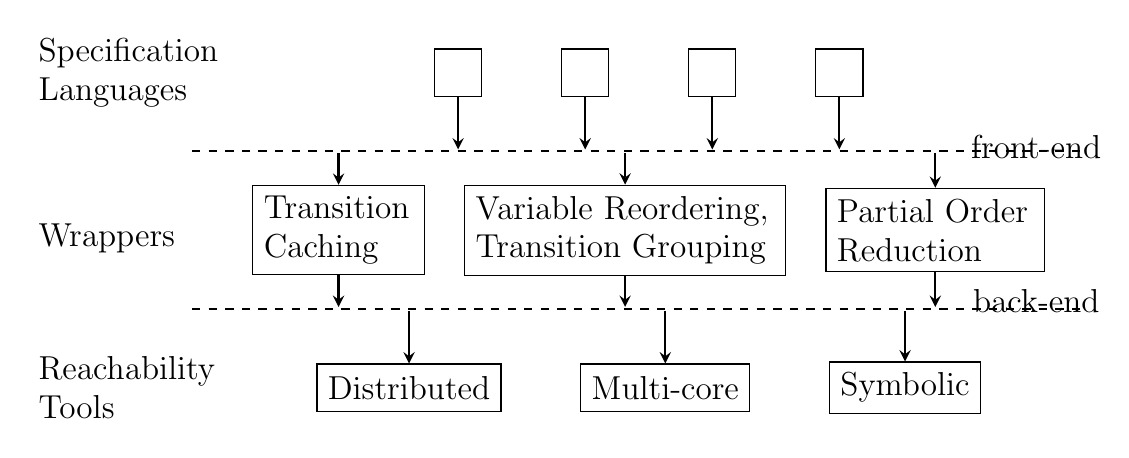
\begin{tikzpicture}[node distance=2cm]
	\large
    \begin{scope}[yshift=4cm]
        \node[node distance=2cm, text width=2.5cm] (speclan) {Specification Languages};
        \node[below of=speclan, node distance=2cm, text width=2.5cm] (p2p) {\pinspins\\ Wrappers};
        \node[below of=p2p, node distance=2cm, text width=2.5cm] (reach) {Reachability Tools};
    \end{scope}    
    
    \begin{scope}[yshift=4cm, xshift=6.5cm]
        \matrix[nodes={draw}, column sep=1cm]{
            \node[minimum size=6mm] (mcrl2) {\mcrl}; &
            \node[minimum size=6mm] (promela) {\promela}; &
            \node[minimum size=6mm] (other) {\dve}; &
            \node[minimum size=6mm] (prob) {\uppaal}; \\
        };
        \node[right of=prob, node distance=2.5cm] (placeholder) {};
        \node[below of=placeholder, node distance=0.95cm, inner sep=0cm] {front-end};
        \node[below of=placeholder, node distance=2.9cm, inner sep=0cm] {back-end};
        
        \node[below of=mcrl2, node distance=1cm, inner sep=0cm] (a) {};
        \node[below of=promela, node distance=1cm, inner sep=0cm] (b) {};
        \node[below of=other, node distance=1cm, inner sep=0cm] (c) {};
        \node[below of=prob, node distance=1cm, inner sep=0cm] (d) {};
        
        \draw (mcrl2) edge[thick, -stealth] (a);
        \draw (promela) edge[thick, -stealth] (b);
        \draw (other) edge[thick, -stealth] (c);
        \draw (prob) edge[thick, -stealth] (d);
    \end{scope}
    
    \draw[thick, dashed](.7,3cm)--(12,3cm);

    \begin{scope}[yshift=2cm, xshift=6.5cm]
        \matrix[nodes={draw}, column sep=.5cm]{
            \node[text width=1.9cm, minimum size=10mm] (cach) {Transition Caching}; &
            \node[text width=3.8cm, minimum size=10mm] (reord) {Variable Reordering, Transition Grouping}; &
            \node[text width=2.5cm, minimum size=10mm] (por) {Partial Order Reduction}; \\
        };
        \node[above of=cach, node distance=1cm, inner sep=0cm] (a) {};
        \node[above of=reord, node distance=1cm, inner sep=0cm] (b) {};
        \node[above of=por, node distance=1cm, inner sep=0cm] (c) {};
        
        \node[below of=cach, node distance=1cm, inner sep=0cm] (d) {};
        \node[below of=reord, node distance=1cm, inner sep=0cm] (e) {};
        \node[below of=por, node distance=1cm, inner sep=0cm] (f) {};
        
        \draw (a) edge[thick, -stealth] (cach);
        \draw (b) edge[thick, -stealth] (reord);
        \draw (c) edge[thick, -stealth] (por);
        
        \draw (cach) edge[thick, -stealth] (d);
        \draw (reord) edge[thick, -stealth] (e);
        \draw (por) edge[thick, -stealth] (f);
    \end{scope}
    
    \draw[thick, dashed](.7,1cm)--(12,1cm);
    
    \begin{scope}[xshift=6.5cm]
        \matrix[nodes={draw}, column sep=1cm]{
            \node[minimum size=6mm] (dist) {Distributed}; &
            \node[minimum size=6mm] (mult) {Multi-core}; &
            \node[minimum size=6mm] (sym) {Symbolic}; \\
        };
        
        \node[above of=dist, node distance=1cm, inner sep=0cm] (a) {};
        \node[above of=mult, node distance=1cm, inner sep=0cm] (b) {};
        \node[above of=sym, node distance=1cm, inner sep=0cm] (c) {};
        
        \draw (a) edge[thick, -stealth] (dist);
        \draw (b) edge[thick, -stealth] (mult);
        \draw (c) edge[thick, -stealth] (sym);
    \end{scope}    
    
\end{tikzpicture}